% !TeX root = ../tfg.tex
% !TeX encoding = utf8

\chapter{Paralelismo}\label{chap:paralel}

El \textit{paralelismo} o \textit{concurrencia} en el proceso de aprendizaje de las redes es el elemento clave a la
hora de minimizar el tiempo de ejecución del entrenamiento de los modelos. Un programa puede, normalmente, dividirse
en muchos componentes que denominamos \textit{tareas}. Un \textit{programa concurrente} es aquel que consiste en un
número de tareas computacionales que pueden ser ejecutadas paralelamente. El programa concurrente define cómo las 
tareas se comunican y cooperan entre sí, además de sincronizar, o no, sus acciones \cite{czech_2017}. 

\vspace{10pt}
Supongamos que tenemos un programa $O$ con siete tareas $o_i$. Es fácil ver cómo el paralelizar procesos ahorra tiempo
de ejecución, como se muestra en las figuras \ref{fig:prog-sec} y \ref{fig:prog-par} (donde $p$ denota procesador).
Podemos observar que, al ser ejecutados de forma simultánea, algunas de las tareas se solapan en el tiempo, acortando 
el tiempo total necesario para la computación del programa \cite{czech_2017}.

\begin{figure}[htbp!]
    \centering
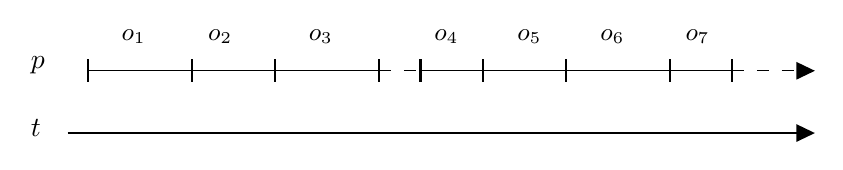
\begin{tikzpicture}[x=0.75pt,y=0.75pt,yscale=-1,xscale=1]
%uncomment if require: \path (0,300); %set diagram left start at 0, and has height of 300
%Straight Lines [id:da7449676638708221] 
\draw    (50,50) -- (72.42,50) -- (100,50) ;
\draw [shift={(100,50)}, rotate = 180] [color={rgb, 255:red, 0; green, 0; blue, 0 }  ][line width=0.75]    (0,5.59) -- (0,-5.59)   ;
\draw [shift={(50,50)}, rotate = 180] [color={rgb, 255:red, 0; green, 0; blue, 0 }  ][line width=0.75]    (0,5.59) -- (0,-5.59)   ;
%Straight Lines [id:da9687422174007011] 
\draw    (100,50) -- (122.42,50) -- (140,50) ;
\draw [shift={(140,50)}, rotate = 180] [color={rgb, 255:red, 0; green, 0; blue, 0 }  ][line width=0.75]    (0,5.59) -- (0,-5.59)   ;
\draw [shift={(100,50)}, rotate = 180] [color={rgb, 255:red, 0; green, 0; blue, 0 }  ][line width=0.75]    (0,5.59) -- (0,-5.59)   ;
%Straight Lines [id:da27287006149854454] 
\draw    (140,50) -- (162.42,50) -- (190,50) ;
\draw [shift={(190,50)}, rotate = 180] [color={rgb, 255:red, 0; green, 0; blue, 0 }  ][line width=0.75]    (0,5.59) -- (0,-5.59)   ;
\draw [shift={(140,50)}, rotate = 180] [color={rgb, 255:red, 0; green, 0; blue, 0 }  ][line width=0.75]    (0,5.59) -- (0,-5.59)   ;
%Straight Lines [id:da5536134933880722] 
\draw    (210,50) -- (232.42,50) -- (240,50) ;
\draw [shift={(240,50)}, rotate = 180] [color={rgb, 255:red, 0; green, 0; blue, 0 }  ][line width=0.75]    (0,5.59) -- (0,-5.59)   ;
\draw [shift={(210,50)}, rotate = 180] [color={rgb, 255:red, 0; green, 0; blue, 0 }  ][line width=0.75]    (0,5.59) -- (0,-5.59)   ;
%Straight Lines [id:da753886597033629] 
\draw    (240,50) -- (262.42,50) -- (280,50) ;
\draw [shift={(280,50)}, rotate = 180] [color={rgb, 255:red, 0; green, 0; blue, 0 }  ][line width=0.75]    (0,5.59) -- (0,-5.59)   ;
\draw [shift={(240,50)}, rotate = 180] [color={rgb, 255:red, 0; green, 0; blue, 0 }  ][line width=0.75]    (0,5.59) -- (0,-5.59)   ;
%Straight Lines [id:da5516104166014002] 
\draw    (280,50) -- (302.42,50) -- (305.58,50) -- (330,50) ;
\draw [shift={(330,50)}, rotate = 180] [color={rgb, 255:red, 0; green, 0; blue, 0 }  ][line width=0.75]    (0,5.59) -- (0,-5.59)   ;
\draw [shift={(280,50)}, rotate = 180] [color={rgb, 255:red, 0; green, 0; blue, 0 }  ][line width=0.75]    (0,5.59) -- (0,-5.59)   ;
%Straight Lines [id:da8194201143798694] 
\draw    (330,50) -- (352.42,50) -- (360,50) ;
\draw [shift={(360,50)}, rotate = 180] [color={rgb, 255:red, 0; green, 0; blue, 0 }  ][line width=0.75]    (0,5.59) -- (0,-5.59)   ;
\draw [shift={(330,50)}, rotate = 180] [color={rgb, 255:red, 0; green, 0; blue, 0 }  ][line width=0.75]    (0,5.59) -- (0,-5.59)   ;
%Straight Lines [id:da65503157723167] 
\draw  [dash pattern={on 4.5pt off 4.5pt}]  (360,50) -- (397,50) ;
\draw [shift={(400,50)}, rotate = 180] [fill={rgb, 255:red, 0; green, 0; blue, 0 }  ][line width=0.08]  [draw opacity=0] (8.93,-4.29) -- (0,0) -- (8.93,4.29) -- cycle    ;
%Straight Lines [id:da7036502375733221] 
\draw    (40,80) -- (397,80) ;
\draw [shift={(400,80)}, rotate = 180] [fill={rgb, 255:red, 0; green, 0; blue, 0 }  ][line width=0.08]  [draw opacity=0] (8.93,-4.29) -- (0,0) -- (8.93,4.29) -- cycle    ;
%Straight Lines [id:da7413442953095534] 
\draw  [dash pattern={on 4.5pt off 4.5pt}]  (190,50) -- (210,50) ;

% Text Node
\draw (21,42) node [anchor=north west][inner sep=0.75pt]   [align=left] {$\displaystyle p$};
% Text Node
\draw (73.83,38.13) node [anchor=south] [inner sep=0.75pt]  [font=\small] [align=left] {$\displaystyle o_{1} \ $};
% Text Node
\draw (115.5,38) node [anchor=south] [inner sep=0.75pt]  [font=\small] [align=left] {$\displaystyle o_{2} \ $};
% Text Node
\draw (164,38) node [anchor=south] [inner sep=0.75pt]  [font=\small] [align=left] {$\displaystyle o_{3} \ $};
% Text Node
\draw (224.5,38) node [anchor=south] [inner sep=0.75pt]  [font=\small] [align=left] {$\displaystyle o_{4} \ $};
% Text Node
\draw (264.5,38) node [anchor=south] [inner sep=0.75pt]  [font=\small] [align=left] {$\displaystyle o_{5} \ $};
% Text Node
\draw (304.5,38) node [anchor=south] [inner sep=0.75pt]  [font=\small] [align=left] {$\displaystyle o_{6} \ $};
% Text Node
\draw (345.5,38) node [anchor=south] [inner sep=0.75pt]  [font=\small] [align=left] {$\displaystyle o_{7} \ $};
% Text Node
\draw (21,72) node [anchor=north west][inner sep=0.75pt]   [align=left] {$\displaystyle t$};
\end{tikzpicture}
    \caption{Programa ejecutado en un procesador $p$ secuencialmente.}
    \label{fig:prog-sec}
\end{figure}

\begin{figure}[htbp!]
    \centering
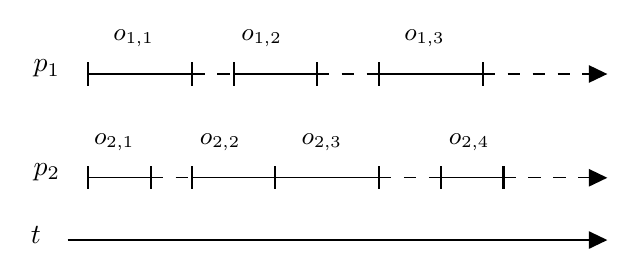
\begin{tikzpicture}[x=0.75pt,y=0.75pt,yscale=-1,xscale=1]
%uncomment if require: \path (0,300); %set diagram left start at 0, and has height of 300

%Straight Lines [id:da7449676638708221] 
\draw    (50,50) -- (72.42,50) -- (100,50) ;
\draw [shift={(100,50)}, rotate = 180] [color={rgb, 255:red, 0; green, 0; blue, 0 }  ][line width=0.75]    (0,5.59) -- (0,-5.59)   ;
\draw [shift={(50,50)}, rotate = 180] [color={rgb, 255:red, 0; green, 0; blue, 0 }  ][line width=0.75]    (0,5.59) -- (0,-5.59)   ;
%Straight Lines [id:da9687422174007011] 
\draw    (120,50) -- (142.42,50) -- (160,50) ;
\draw [shift={(160,50)}, rotate = 180] [color={rgb, 255:red, 0; green, 0; blue, 0 }  ][line width=0.75]    (0,5.59) -- (0,-5.59)   ;
\draw [shift={(120,50)}, rotate = 180] [color={rgb, 255:red, 0; green, 0; blue, 0 }  ][line width=0.75]    (0,5.59) -- (0,-5.59)   ;
%Straight Lines [id:da27287006149854454] 
\draw    (190,50) -- (212.42,50) -- (240,50) ;
\draw [shift={(240,50)}, rotate = 180] [color={rgb, 255:red, 0; green, 0; blue, 0 }  ][line width=0.75]    (0,5.59) -- (0,-5.59)   ;
\draw [shift={(190,50)}, rotate = 180] [color={rgb, 255:red, 0; green, 0; blue, 0 }  ][line width=0.75]    (0,5.59) -- (0,-5.59)   ;
%Straight Lines [id:da7036502375733221] 
\draw    (40,130) -- (297,130) ;
\draw [shift={(300,130)}, rotate = 180] [fill={rgb, 255:red, 0; green, 0; blue, 0 }  ][line width=0.08]  [draw opacity=0] (8.93,-4.29) -- (0,0) -- (8.93,4.29) -- cycle    ;
%Straight Lines [id:da6774992036569548] 
\draw    (50,100) -- (72.42,100) -- (80,100) ;
\draw [shift={(80,100)}, rotate = 180] [color={rgb, 255:red, 0; green, 0; blue, 0 }  ][line width=0.75]    (0,5.59) -- (0,-5.59)   ;
\draw [shift={(50,100)}, rotate = 180] [color={rgb, 255:red, 0; green, 0; blue, 0 }  ][line width=0.75]    (0,5.59) -- (0,-5.59)   ;
%Straight Lines [id:da40797715400302237] 
\draw    (100,100) -- (122.42,100) -- (140,100) ;
\draw [shift={(140,100)}, rotate = 180] [color={rgb, 255:red, 0; green, 0; blue, 0 }  ][line width=0.75]    (0,5.59) -- (0,-5.59)   ;
\draw [shift={(100,100)}, rotate = 180] [color={rgb, 255:red, 0; green, 0; blue, 0 }  ][line width=0.75]    (0,5.59) -- (0,-5.59)   ;
%Straight Lines [id:da9796982630377253] 
\draw    (140,100) -- (162.42,100) -- (165.58,100) -- (190,100) ;
\draw [shift={(190,100)}, rotate = 180] [color={rgb, 255:red, 0; green, 0; blue, 0 }  ][line width=0.75]    (0,5.59) -- (0,-5.59)   ;
\draw [shift={(140,100)}, rotate = 180] [color={rgb, 255:red, 0; green, 0; blue, 0 }  ][line width=0.75]    (0,5.59) -- (0,-5.59)   ;
%Straight Lines [id:da12074639444172841] 
\draw    (220,100) -- (242.42,100) -- (250,100) ;
\draw [shift={(250,100)}, rotate = 180] [color={rgb, 255:red, 0; green, 0; blue, 0 }  ][line width=0.75]    (0,5.59) -- (0,-5.59)   ;
\draw [shift={(220,100)}, rotate = 180] [color={rgb, 255:red, 0; green, 0; blue, 0 }  ][line width=0.75]    (0,5.59) -- (0,-5.59)   ;
%Straight Lines [id:da9578737855209709] 
\draw  [dash pattern={on 4.5pt off 4.5pt}]  (250,100) -- (297,100) ;
\draw [shift={(300,100)}, rotate = 180] [fill={rgb, 255:red, 0; green, 0; blue, 0 }  ][line width=0.08]  [draw opacity=0] (8.93,-4.29) -- (0,0) -- (8.93,4.29) -- cycle    ;
%Straight Lines [id:da7283794267429679] 
\draw  [dash pattern={on 4.5pt off 4.5pt}]  (240,50) -- (297,50) ;
\draw [shift={(300,50)}, rotate = 180] [fill={rgb, 255:red, 0; green, 0; blue, 0 }  ][line width=0.08]  [draw opacity=0] (8.93,-4.29) -- (0,0) -- (8.93,4.29) -- cycle    ;
%Straight Lines [id:da5907876233465004] 
\draw  [dash pattern={on 4.5pt off 4.5pt}]  (100,50) -- (120,50) ;
%Straight Lines [id:da21619386708455546] 
\draw  [dash pattern={on 4.5pt off 4.5pt}]  (80,100) -- (100,100) ;
%Straight Lines [id:da015175278052757313] 
\draw  [dash pattern={on 4.5pt off 4.5pt}]  (160,50) -- (190,50) ;
%Straight Lines [id:da8933562725547656] 
\draw  [dash pattern={on 4.5pt off 4.5pt}]  (190,100) -- (220,100) ;

% Text Node
\draw (30,42) node [anchor=north] [inner sep=0.75pt]   [align=left] {$\displaystyle p_{1}$};
% Text Node
\draw (73.83,38.13) node [anchor=south] [inner sep=0.75pt]  [font=\small] [align=left] {$\displaystyle o_{1,1} \ $};
% Text Node
\draw (135.5,38) node [anchor=south] [inner sep=0.75pt]  [font=\small] [align=left] {$\displaystyle o_{1,2} \ $};
% Text Node
\draw (214,38) node [anchor=south] [inner sep=0.75pt]  [font=\small] [align=left] {$\displaystyle o_{1,3} \ $};
% Text Node
\draw (21,122) node [anchor=north west][inner sep=0.75pt]   [align=left] {$\displaystyle t$};
% Text Node
\draw (29.98,92) node [anchor=north] [inner sep=0.75pt]   [align=left] {$\displaystyle p_{2}$};
% Text Node
\draw (64.5,88) node [anchor=south] [inner sep=0.75pt]  [font=\small] [align=left] {$\displaystyle o_{2,1} \ $};
% Text Node
\draw (115.5,88) node [anchor=south] [inner sep=0.75pt]  [font=\small] [align=left] {$\displaystyle o_{2,2} \ $};
% Text Node
\draw (164.5,88) node [anchor=south] [inner sep=0.75pt]  [font=\small] [align=left] {$\displaystyle o_{2,3} \ $};
% Text Node
\draw (235.5,88) node [anchor=south] [inner sep=0.75pt]  [font=\small] [align=left] {$\displaystyle o_{2,4} \ $};


\end{tikzpicture}
    \caption{Programa ejecutado en dos procesadores $p_1$ y $p_2$ paralelamente.}
    \label{fig:prog-par}
\end{figure}

\vspace{10pt}
Durante este capítulo vamos a estudiar algunos conceptos básicos del paralelismo y medidas para comprobar su 
efectividad. Hablaremos también de Spark, un motor analítico y marco de trabajo desarrollado por Apache para el 
procesamiento de grandes cantidades de datos utilizando como soporte GPUs conectadas en red. 

\vspace{10pt}
Denotaremos el número de procesadores o procesos con $p$ y llamaremos ``multiprocesador'' a cualquier computadora 
que contenga más de un procesador \cite{wilkinson_allen_2005}.

% -------------------------------------------------------------------------------------------------------------------
\section{Velocidad computacional}

La primera gran pregunta que se puede hacer a la hora de desarrollar un programa concurrente es cuánta velocidad de
computación se gana con esa solución en lugar de una secuencial. Para hacer esta comparativa, tomamos como base el
tiempo de ejecución del mejor algoritmo secuencial ($t_s$) contra el tiempo de ejecución de la solución paralela
utilizando $p$ procesadores ($t_p$). La \textit{\textbf{speedup factor}}, o \textit{\textbf{factor de aceleración}} es 
una medida de rendimiento relativo, definida como:
\begin{equation}\label{eq:speedup}
    S(p)=\frac{t_s}{t_p}
\end{equation}
Esta medida representa el ratio de mejora de la velocidad de ejecución utilizando un multiprocesador. Es importante 
notar que no siempre el algoritmo secuencial coincidirá con el concurrente; de hecho, lo más probable es que no sea
así \cite{wilkinson_allen_2005}.

\vspace{10pt}
El valor máximo del factor de aceleración suele ser $p$, y se le llama \textbf{\textit{aceleración lineal}}. Esta
aceleración se conseguiría si las tareas del algoritmo secuencial se pudiesen dividir perfectamente en procesos de
misma duración, y asignar cada uno de ellos a cada uno de los procesadores, sin ningún tiempo añadido por sobrecargas o
computaciones iniciales relativas a la paralelización. De esta manera, tenemos que:
\begin{equation}
    S(p)\leq\frac{t_s}{^{t_s}/_{p}}=p
\end{equation}
Es posible obtener \textbf{\textit{aceleración superlineal}}, es decir, $S(p)>p$, si el algoritmo secuencial no es el
óptimo, si el multiprocesador contiene una característica especial en cuanto a arquitectura que favorezca la 
paralelización, por el aumento de memoria utilizable al utilizar múltiples procesadores o por factores de 
indeterminismo de los algoritmos utilizados. Generalmente, si ocurre este tipo de aceleración, significa que el
programa concurrente puede ser simulado en un único procesador ejecutando los procesos paralelos de forma secuencial, 
lo que sugiere que el algoritmo secuencial utilizado para la comparativa no es el adecuado \cite{wilkinson_allen_2005}.

\vspace{10pt}
Otra medida interesante a la hora de comparar los algoritmos secuenciales y los concurrentes es la 
\textbf{\textit{eficiencia}}. Esta medida nos muestra cuánto tiempo están en uso los procesadores durante la 
computación. Se define como:
\begin{equation}
    E=\frac{t_s}{t_p\cdot p}=\frac{S(p)}{p}
\end{equation}
Podemos ver la eficiencia como un porcentaje. Cuando $E=1$ ($E=100\%$), entonces es porque los procesadores están 
siendo utilizados durante todo el tiempo de ejecución del algoritmo y tenemos aceleración lineal 
\cite{wilkinson_allen_2005}.

% -------------------------------------------------------------------------------------------------------------------
\subsection{Ley de Amdahl}

Una vez que tenemos una medida para la ganancia de velocidad, cabe preguntarse cuál es la ganancia máxima posible.
Existen factores en los algoritmos concurrentes que crean sobrecargas de computación, como pueden ser: Tiempo de
comunicación entre los distintos procesos, computaciones adicionales necesarias en el algoritmo concurrente que no
ocurren en el secuencial, como el cálculo de constantes locales o los periodos de tiempo en los cuales no todos los
procesos están realizando tareas de computación \cite{wilkinson_allen_2005}.

\begin{figure}[htbp!]
    \centering
    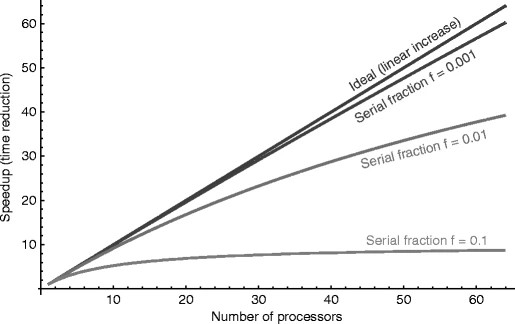
\includegraphics[width=0.7\textwidth]{img/amdahl.jpg}
    \caption{Factor de aceleración dependiendo de la fracción secuencial, según la ley de Amdahl \cite{Gustafson2011}}
    \label{fig:amdahl}
\end{figure}

\vspace{10pt}
Es razonable esperar que parte de las tareas computacionales no puedan ser divididas en procesos paralelos, teniendo
que ser ejecutadas secuencialmente. Supongamos que existe un periodo durante el cual únicamente está siendo utilizado 
un procesador, por ejemplo, un periodo de inicialización en el cual se están generando las posteriores tareas 
paralelas. A partir de esta asunción, lo ideal es que el resto de tareas sean realizadas por todos los procesadores 
disponibles trabajando simultáneamente. Si denotamos por $f$ a la fracción de la computación no paralelizable y $t_s$ 
al tiempo de ejecución del algoritmo secuencial, tenemos que el factor de aceleración es:
\begin{equation}\label{eq:ley-amdahl}
    S(p)=\frac{t_s}{f\cdot t_s+\displaystyle\frac{(1-f)t_s}{p}}=\frac{p}{1+(p-1)f}
\end{equation}
Esta ecuación es conocida como \textit{\textbf{ley de Amdahl}} \cite{wilkinson_allen_2005}. Esta ley nos hace inferir 
que el factor más importante a la hora de considerar la concurrencia es qué fracción de la computación es  
paralelizable, ya que, aún teniendo un número infinito de procesadores, la ganancia obtenida máxima será
\begin{equation}
    \lim_{p\to\infty} S(p)=\lim_{p\to\infty} \frac{p}{1+(p-1)f}=\frac{1}{f}
\end{equation}
Podemos ver este comportamiento de manera gráfica en la figura \ref{fig:amdahl}. Es importante notar que esta ecuación
es únicamente útil cuando la cantidad de tareas computacionales es fija.

% -------------------------------------------------------------------------------------------------------------------
\section{Escalabilidad}

No siempre un aumento de los procesadores tiene por qué implicar una mejora proporcional, como hemos visto a través de
la ley de Amdahl. Uno de los factores importantes a la hora de utilizar programas concurrentes es la escalabilidad.

\vspace{10pt}
Este término es, sin embargo, impreciso. Suele utilizarse para indicar en el diseño \textit{hardware} si un sistema,
al aumentar su tamaño, aumenta también su rendimiento. La escalabilidad también se utiliza para indicar si un algoritmo
paralelo, al aumentar el número de datos de entrada o trabajo computacional no aumenta de forma desproporcionada el
aumento de etapas de computación. Cuando se utiliza en este sentido, se le denomina 
\textbf{\textit{escalabilidad algorítmica}} \cite{wilkinson_allen_2005}. 

\vspace{10pt}
Para estudiar la escalabilidad de los algoritmos concurrentes, la ley de Amdahl no proporciona la información 
suficiente, por lo que es necesario utilizar otras medidas.

% -------------------------------------------------------------------------------------------------------------------
\subsubsection*{Ley de Gustafson}

El primer supuesto de la ley de Amdahl es la suposición de que la cantidad de trabajo computacional es fija. Esta
suposición es útil, puesto que evita definir el trabajo computacional, pero no tiene en cuenta que se puede buscar una
mejora computacional en lugar de una mejora temporal mediante la paralelización \cite{Gustafson2011}. 

\vspace{10pt}
En la práctica, la paralelización suele utilizarse para realizar tareas de computación mucho más grandes para que 
mantengan un tiempo de ejecución razonable, para lo cual necesitamos una medida que tenga en cuenta este factor, y que 
nos dará alguna medida de la escalabilidad algorítmica de los modelos utilizados. Por tanto, es válido asumir que el 
tiempo de ejecución del algoritmo es fijo, siendo la cantidad de trabajo computacional o tamaño de los datos de entrada 
la que varía entre la versión secuencial y la paralela. Utilizando este supuesto, el factor de aceleración será 
numéricamente distinto a los calculados anteriormente, y se le llama \textbf{\textit{factor de aceleración escalado}}, 
y fue formulado por Gustafson en 1988. En esta ecuación, es el tiempo de ejecución paralelo el que es constante, en 
lugar del secuencial \cite{wilkinson_allen_2005}. La ecuación, llamada usualmente \textbf{\textit{ley de Gustafson}}, 
tiene la forma
\begin{equation}
    S_s(p)=p+(1-p)f\cdot t_s=p-f(p-1)
\end{equation}

% -------------------------------------------------------------------------------------------------------------------
\subsubsection*{Paralelismo parcial}

No siempre un algoritmo puede paralelizar todas sus tareas de forma que se utilice el total de los procesadores 
disponibles, sino que puede haber diferentes grados de paralelización para sus diferentes tareas, como por ejemplo, los
algoritmos que utilizan técnicas como ``divide y vencerás'' \cite{SUN199327}. El modelo de Amdahl
no contempla este tipo de situaciones. Una ecuación más realista y detallada en la cual el paralelismo puede variar 
entre $1$ y $n$ procesadores es:
\begin{equation}
    S(n)=\frac{1}{f_1+\displaystyle\frac{f_2}2+\displaystyle\frac{f_3}3+\cdots+\displaystyle\frac{f_n}n}
\end{equation}
donde $f_i$ es la fracción del algoritmo que puede ser ejecutada por $i$ procesadores en paralelo, y $f_1+\cdots+f_n=1$
\cite{Gustafson2011}.

% -------------------------------------------------------------------------------------------------------------------
\subsubsection*{Comunicación entre procesos}

\vspace{10pt}
Debido al momento histórico de la formulación de la ley por Gene Amdahl, 1967, el coste de comunicación entre los
procesadores se estimó como insignificante. Esto fue así debido a que en ese momento la computación de los algoritmos
era magnitudes superiores en cuanto a tiempo que la comunicación entre los procesadores. La velocidad de computación
de los procesadores modernos es mucho mayor que la velocidad de comunicación de datos entre los mismos
\cite{Gustafson2011}.

\vspace{10pt}
Si denominamos $t_{\text{cm}}$ al tiempo de ejecución gastado en la comunicación entre los diferentes procesadores
y $t_{\text{cp}}$, podemos establecer una nueva medida, a la que llamaremos 
\textbf{\textit{ratio computación/comunicación}}, calculado como:
\begin{equation}
    R_{cc}=\frac{t_{\text{cp}}}{t_{\text{cm}}}
\end{equation}
Supongamos que disponemos de $p$ procesadores y $n$ elementos de datos para un algoritmo. El ratio nos permite conocer
el potencial de escalabilidad del algoritmo. Supongamos, por ejemplo, que para un valor $p$, tenemos que nuestro
algoritmo requiere $c_1n$ computaciones y $c_2n^2$ comunicaciones. 

\vspace{10pt}
Utilizando el ratio computación/comunicación, podemos ver que la paralelización no mejora sustancialmente el tiempo de 
ejecución del programa conforme va aumentando el número de elementos de datos, puesto que:
\begin{equation}
    R_{cc}=\frac{c_1n}{c_2n^2}=\frac{c_1}{c_2n}\Rightarrow\lim_{n\to\infty} R_{cc}=0
\end{equation}
Normalmente, vamos a preferir aquellas soluciones que maximicen el ratio computación/comunicación, es decir, aquellos
que transformen $R_{cc}$ es una función creciente respecto a $n$. Es importante notar que para obtener esta medida,
es necesario ejecutar el programa primero, calculando después el ratio \cite{wilkinson_allen_2005}.

% -------------------------------------------------------------------------------------------------------------------
\section{Clústeres}

Una de las formas de obtener un multiprocesador es el uso de \textbf{\textit{clústeres}}, que no es más que duplicar
unidades procesamiento y combinarlas. Los clústeres se conciben como sistemas de computación paralela constituidos por
\textbf{\textit{nodos}} interconectados, compuestos por procesadores, memorias, buses, \dots; que cooperan entre sí.
Los nodos se comunican entre sí mediante el paso de mensajes. Dependiendo de los componentes de la arquitectura, se 
pueden definir distintos tipos de clústeres \cite{czech_2017}.

\begin{figure}[htbp!]
    \centering
    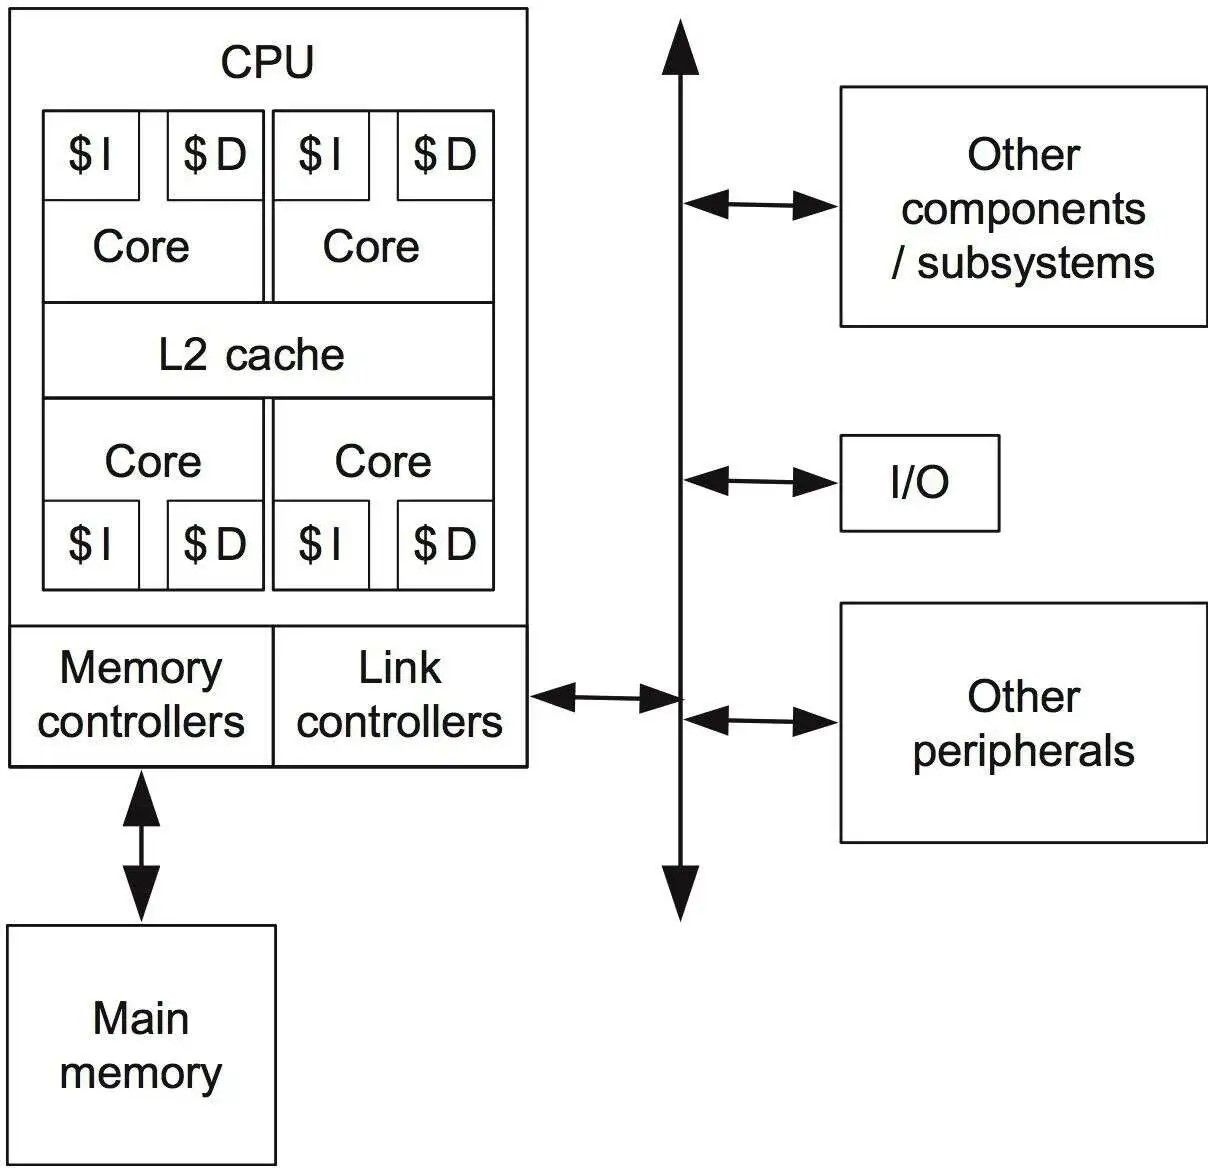
\includegraphics[width=0.6\textwidth]{img/MCP.jpg}
    \caption{Arquitectura de clúster de procesador con cuatro núcleos \cite{mcp}.}
    \label{fig:mcp}
\end{figure}

% -------------------------------------------------------------------------------------------------------------------
\subsection{Procesador multinúcleo}

La estructura de este tipo de clústeres se basa en la unión de varias unidades de procesamiento separadas, denominadas
núcleos, en un único chip. De esta manera, se puede construir una máquina capaz de ejecutar diferentes tareas de
computación en diferentes partes de la memoria. La memoria en este clúster es común para todos nodos (núcleos), así 
como el resto de componentes de la máquina. La mayoría de computadores actualmente presentan esta arquitectura. Un 
esquema de este tipo de clúster es el de la figura \ref{fig:mcp}.

\vspace{10pt}
Debido a que este tipo de clústeres la mayor parte de la computación y comunicación se realiza sobre memoria 
compartida, son más adecuados para implementar algoritmos de granularidad fina y con referencias a datos diversas, es
decir, datos locales y no locales \cite{czech_2017}.

% -------------------------------------------------------------------------------------------------------------------
\subsection{Clúster de computadores}

Un clúster de computadores se construye conectando mediante una red una cierta cantidad de computadores, conformando
cada uno de ellos un nodo. Si los computadores son idénticos en términos de arquitectura, hardware y software, se dice
que el clúster es \textit{homogéneo} \cite{czech_2017}. Es posible combinar varias arquitecturas, es decir, podemos
tener un clúster de computadores conformado por máquinas con procesadores multinúcleo.

\vspace{10pt}
El uso de una red de computadores tiene ventajas sobre el uso de sistemas multiprocesadores específicos. Las ventajas
clave son:
\begin{enumerate}
    \item Los PCs o estaciones de trabajo de grandes prestaciones son fáciles de adquirir a un bajo coste.
    \item Los procesadores pueden ser sustituidos conforme otros con mejores prestaciones van apareciendo, y el clúster 
    puede cambiar de tamaño fácilmente, aumentando o disminuyendo el número de máquinas.
    \item Es posible utilizar aplicaciones software existentes sobre el clúster.
\end{enumerate}
\begin{figure}[htbp!]
    \centering
    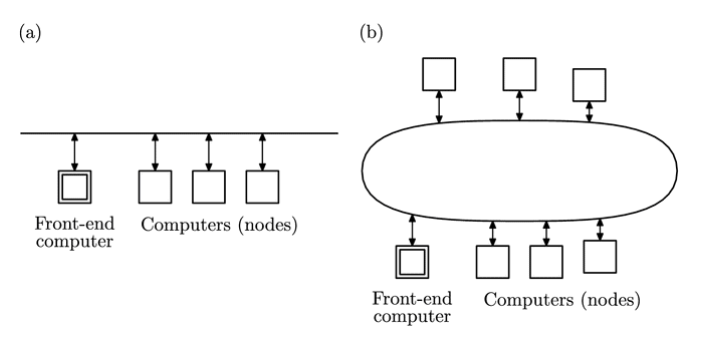
\includegraphics[width=0.8\textwidth]{img/cluster.png}
    \caption{Clúster de computadores: conectados mediante un único cable de red (a) o con una topología de anillo (b). En ambos casos, un nodo \textit{front-end} se encarga de la gestión del clúster \cite{czech_2017}.}
    \label{fig:cluster}
\end{figure}

\vspace{10pt}
El caso más común de clúster de computadores es la conexión mediante cables Ethernet de computadores mediante diversas
topologías de red, como se muestra en la figura \ref{fig:cluster}. El primero de ellos fue construido en 1994 en el 
Centro de Vuelo Espacial Goddard de la NASA, en el cual se conectaron los ordenadores personales de los ingenieros. 
Sus creadores lo denominaron Beowulf a raíz del héroe legendario medieval. Podemos decir que este tipo de clústeres 
son \textit{centralizados}, mientras que los denominados \textit{descentralizados} suelen estar conformados por nodos 
separados físicamente y conectados mediante Internet, donde cada nodo puede ser reconfigurado, encendido o apagado en 
cualquier momento \cite{czech_2017}.

% -------------------------------------------------------------------------------------------------------------------
\subsection{Memoria compartida distribuida}

Uno de los problemas que puede acarrear un clúster de computadores centralizado es la formación de un cuello de 
botella en el paso de información, ya que el acceso a la memoria y el paso de mensajes se realiza a través de un canal 
de red.  La \textbf{\textit{memoria compartida distribuida}} (DSM) es una posible solución a este problema. Esta 
arquitectura, apreciable en la figura \ref{fig:dsm}, ofrece un espacio de direcciones virtual compartido por todos los 
nodos de la red, evitando así la necesidad de paso de mensajes entre los distintos procesadores \cite{nitzberg_91}.

\begin{figure}[htbp!]
    \centering
    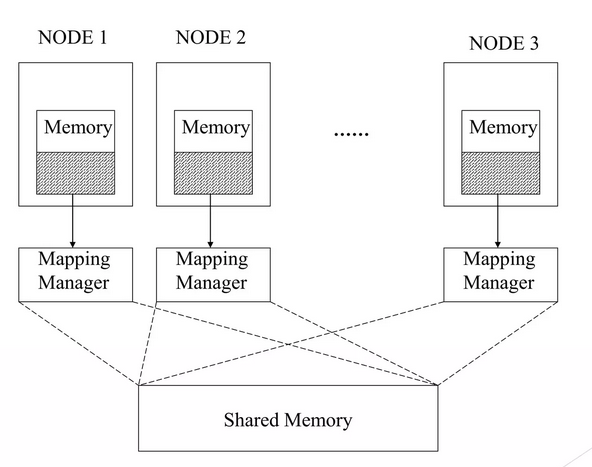
\includegraphics[width=0.6\textwidth]{img/dsm.png}
    \caption{Arquitectura de memoria compartida distribuida \cite{dsm}.}
    \label{fig:dsm}
\end{figure}

\vspace{10pt}
Las ventajas de esta arquitectura frente tanto a un clúster de computadores usual o a un multiprocesador con memoria 
compartida son las siguientes:
\begin{itemize}
    \item Suele resultar más natural programar algoritmos concurrentes utilizando memoria compartida en lugar de paso
    de mensajes explícito. En ocasiones, como puede ser estructuras que contengan punteros, puede llegar a ser incluso
    imposible.
    \item La mayoría de programas están escritos para ser ejecutados en multiprocesadores con memoria compartida 
    (procesadores multinúcleo). Los sistemas DSM permiten ejecutar ese tipo de programas.
    \item Algoritmos que requieran grandes cantidades de memoria pueden ser ejecutados sin problema en esta 
    arquitectura, ya que los procesadores tienen acceso a una gran cantidad de memoria compartida.
    \item El intercambio de datos a través de bloques de memoria es más eficiente que el paso de información a través
    de mensajes.
\end{itemize}
Uno de los problemas principales de esta arquitectura es la gestión de la heterogeneidad entre los distintos nodos de
la red. Al tener memoria compartida, puede suponer grandes costes computacionales la transformación de los datos si
los nodos tienen diferentes formas de representación de los mismos \cite{nitzberg_91}.

% -------------------------------------------------------------------------------------------------------------------
\section{Spark}

La herramienta utilizada para realizar la paralelización en este trabajo es Spark. Esta herramienta se puede utilizar
tanto en en clústeres de ordenadores como un en un clúster independiente, es decir, una sola máquina. Forma parte 
de la \textit{Apache Software Foundation}, una organización sin ánimo de lucro responsable de algunos de los proyectos 
de software libre más importantes. Basada en los RDDs, \textit{resilient distributed datasets}, descritos por Matei 
Zaharia y otros en la Universidad de California, Spark es la herramienta más utilizada para realizar tareas 
computacionales escalables y ciencia de datos \cite{spark}.

% -------------------------------------------------------------------------------------------------------------------
\subsection{RDDs}

Los RDDs, \textit{resilient distributed datasets} o \textbf{\textit{conjuntos de datos resilientes distribuidos}} en
castellano, son estructuras paralelas tolerantes a fallos que permiten la persistencia de resultados intermedios en
memoria, pudiendo manipularlos mediante un conjunto de operadores. Son especialmente útiles para aplicaciones en las
cuales se reutilizan cálculos intermedios a lo largo de múltiples computaciones, como pueden ser la mayoría de 
algoritmos de aprendizaje automático iterativos: regresión logística, $K$-medias, \dots \cite{rdds}

\vspace{10pt}
Formalmente, un RDD es una colección particionada de registros de sólo lectura. Pueden ser creados a partir de 
operaciones deterministas sobre datos en un almacenamiento estable o a partir de otros RDDs. A estas operaciones las
denominaremos \textit{transformaciones} para diferenciarlas del resto de operaciones. Ejemplos de estas 
transformaciones son el mapeo, los filtros y la unión.

\vspace{10pt}
El objetivo principal de los RDDs es definir una interfaz programática que sea capaz de proveer tolerancia a fallos de
forma eficiente. Las arquitecturas de memoria compartida distribuida ofrecen una interfaz basada en actualizaciones
de granularidad fina de estados mutables como por ejemplo, celdas de una tabla. La única manera de proveer tolerancia
a fallos es replicar los datos en otras máquinas o registrar las actualizaciones en los nodos \cite{rdds}. 

\vspace{10pt}
Ambos enfoques son costosos para cargas de trabajo con uso intensivo de datos, puesto que requieren copiar grandes 
cantidades de datos a través de la red del clúster, cuyo ancho de banda suele ser mucho menor que el de la RAM, 
incurriendo en una sobrecarga sustancial de almacenamiento \cite{rdds}.

\vspace{10pt}
A diferencia de esa arquitectura, los RDDs ofrecen una interfaz basada en operaciones de poca granularidad 
(transformaciones) que aplican la misma operación a muchos elementos de datos. Esto les permite tolerar fallos 
registrando las transformaciones utilizadas para construir el conjunto de datos, lo que llamaremos \textit{linaje}, en 
lugar de los datos reales. Si una partición de un RDD se pierde, el RDD tiene información suficiente sobre cómo se 
obtuvo de otros RDDs para volver a calcular sólo esa partición. De esta manera, los datos perdidos pueden recuperarse, 
a menudo con bastante rapidez, sin necesidad de una costosa replicación. Aunque inicialmente pueda parecer limitada una 
interfaz basada en transformaciones de poca granularidad, los RDDs son una buena solución para la mayoría de programas 
paralelos, porque estas aplicaciones realizan de forma natural la misma operación sobre múltitud de datos\cite{rdds}.

\vspace{10pt}
Un RDD no tiene por qué estar materializado en todo momento, más bien al contrario, puesto que contiene suficiente
información acerca de cómo fue construido a través de su linaje para computar sus particiones a partir de los datos
en el almacenamiento estable. En esencia, un programa no puede referenciar un RDD que no sea capaz de reconstruir 
después de un fallo \cite{rdds}.

% -------------------------------------------------------------------------------------------------------------------
\subsubsection*{Ventajas}

Para comprender los beneficios de los RDDs como arquitectura de memoria distribuida, vamos a compararlos con la 
arquitectura de memoria compartida distribuida, cuyo resumen se puede ver en la tabla \ref{tab:rdds}. Para entender la
comparativa, es importante notar que, en los sistemas DSM, las aplicaciones pueden leer y escribir en regiones 
arbitrarias de la memoria global compartida \cite{rdds}.

\vspace{10pt}
La diferencia principal entre las arquitecturas es que los RDDs solamente pueden crearse (lo que viene a ser 
``escribirse'', al ser inmutables) mediante transformaciones, que son de poca granularidad, mientras que la DSM permite
lecturas y escrituras a cualquier región de la memoria. Esto restringe a los RDDs a aplicaciones que realizan 
escrituras en masa, en beneficio de una tolerancia a fallos muy eficiente. En particular, los RDDs no generan 
sobrecargas al no necesitar puntos de control, puesto que pueden reconstruirse a partir de su linaje. Además, sólo las
particiones perdidas de un RDD necesitan recomputarse en caso de fallo, y pueden reconstruirse de forma paralela en
distintos nodos sin tener que hacer una vuelta atrás del programa \cite{rdds}.

\begin{table}[htbp!]
\begin{tabular}{|p{0.25\textwidth}|p{0.32\textwidth}|p{0.32\textwidth}|}
\hline
\multicolumn{1}{|c|}{\textbf{Característica}} & \multicolumn{1}{c|}{\textbf{RDDs}} & \multicolumn{1}{c|}{\textbf{DSM}} \\ \hline
\textit{Lecturas} & Escala completa de granularidad & Granularidad fina \\ \hline
\textit{Escrituras} & Poca granularidad & Granularidad fina \\ \hline
\textit{Consistencia} & Trivial (inmutables) & Responsabilidad de la aplicación o \textit{runtime} \\ \hline
\textit{Recuperación de fallos} & Granularidad fina y poca sobrecarga utilizando el linaje & Requiere puntos de control y vueltas atrás del programa \\ \hline
\textit{Mitigación de rezagados} & Posible utilizando tareas de respaldo & Difícil \\ \hline
\textit{Reparto de tareas} & Automática basada en la localidad de datos & Responsabilidad de la aplicación \\ \hline
\textit{Comportamiento ante sobrecarga} & Similar a otros sistemas de flujos de datos & Bajo rendimiento \\ \hline
\end{tabular}
\caption{Comparativa entre RDDs y memoria compartida distribuida \cite{rdds}.}
\label{tab:rdds}
\end{table}

\vspace{10pt}
Otra de las ventajas que proporcionan los RDDs es su inmutabilidad. Gracias a ella, son capaces de mitigar los nodos
lentos o rezagados lanzando copias de respaldo de las tareas lentas. Estas tareas de respaldo serían muy difíciles de
implementar en DSM, puesto que ambas copias de la tarea accederían a las mismas direcciones de memoria, interfiriendo
en las actualizaciones de cada una \cite{rdds}.

\vspace{10pt}
Finalmente, en operaciones masivas sobre RDDs, un \textit{runtime} reparte y programa las tareas basándose en la 
localidad de los datos para mejorar el rendimiento. Además, para operaciones masivas que sobrecargan el sistema en 
cuanto a memoria, los RDDs se degradan con elegancia siempre y cuando sólo se utilicen en operaciones de escaneo. Las 
particiones que no caben en la memoria se pueden almacenar en el disco y brindan un rendimiento similar al resto de 
sistemas de datos en paralelo \cite{rdds}.

% -------------------------------------------------------------------------------------------------------------------
\subsection{Interfaz}

Spark expone los RDDs mediante una API integrada en el lenguaje Scala, aunque existen librerías actualmente de Spark en
muchos otros lenguajes, como Python. Cada conjunto de datos se representa en esta API como un objeto, y las 
transformaciones se invocan como métodos sobre esos objetos.

\vspace{10pt}
Para programar utilizando RDDs, se comienza definiendo uno o más RDDs mediante transformaciones sobre datos en un
almacenamiento estable. Después se pueden utilizar estos objetos en \textit{acciones}, operaciones que devuelven un
valor a la aplicación o exportan datos a un sistema de almacenamiento. Ejemplos de estas acciones son:
\begin{itemize}
    \item \textit{count}: Devuelve el número de elementos del conjunto de datos.
    \item \textit{collect}: Devuelve los elementos del conjunto de datos explícitamente.
    \item \textit{save}: Guarda los datos en el sistema de almacenamiento.
\end{itemize}
Spark realiza la computación de los RDDs de forma diferida la primera vez que se utilizan en una acción, pudiendo de
esta manera encadenar transformaciones \cite{rdds}.

\vspace{10pt}
Además, se puede llamar a un método de persistencia para indicar qué RDDs se desea reutilizar en operaciones futuras.
Spark mantiene estos objetos en memoria por defecto, pero puede volcarlos al almacenamiento en disco si no queda
suficiente espacio en RAM. También implementa otras estrategias de persistencia, como el almacenamiento del RDD 
únicamente en disco o replicando un RDD en varias máquinas mediante parámetros del método \textit{persist} \cite{rdds}.

\vspace{10pt}
Para utilizar Spark, un programador debe escribir un \textit{programa controlador} que se conecta a un clúster de
\textit{trabajadores}. Este controlador define los RDDs e invoca las acciones sobre ellos. El código de Spark en el
controlador es también el que lleva el linaje de los RDDs. Los trabajadores son procesos de larga duración que 
almacenan las particiones del RDD en la RAM a lo largo de las operaciones \cite{rdds}. El algoritmo de aprendizaje
distribuido implementado en la herramienta sería en este caso el programa controlador, y hablaremos de él en el 
siguiente capítulo.

\endinput
%--------------------------------------------------------------------
% FIN DEL CAPÍTULO. 
%--------------------------------------------------------------------
